\documentclass[residuals.tex]{subfiles}

% Load any packages needed for this document
\begin{document}
\subsection*{Autocorrelation} 
\begin{itemize}
\item Adjacent residuals should not be correlated with each other (\textbf{autocorrelation}). 
\item If you can use one residual to predict the next residual, there is some predictive information present that is not captured by the predictors. 
\item Typically, this situation involves time-ordered observations. 
\end{itemize}

\begin{figure}[h!]
\centering
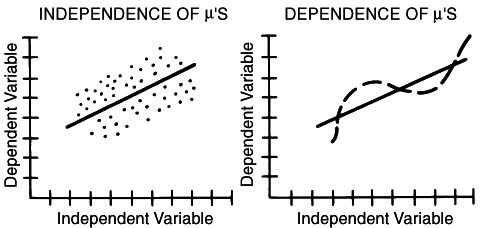
\includegraphics[width=0.7\linewidth]{autocorrelation1}
\caption{(disregard the titles)}

\end{figure}
\begin{itemize}
\item For example, if a residual is more likely to be followed by another residual that has the same sign, adjacent residuals are positively correlated. 
\item You can include a variable that captures the relevant time-related information, or use a time series analysis.
\end{itemize}
 
\newpage
\subsection*{Durbin-Watson Test for Autocorrelated Errors}
The \textbf{\textit{Durbin-Watson} }procedure is commonly used to to test for autocorrelation of residuals. To perform this test, we use the \texttt{durbinWatsonTest()} from the car R package. All you have to do is to specify the name of the fitted mode.

\begin{framed}
\begin{verbatim}

 FitMod <- lm(mpg~wt+cyl,data=mtcars)

# library(car)
durbinWatsonTest(FitMod)

\end{verbatim}
\end{framed}
\begin{itemize}
\item The null hypothesis can simply be stated as "There is no autocorrelation present in the residuals".. 
\item The \texttt{R} code output provides a $p-$value to base a determination on.
\end{itemize}

\begin{framed}
\begin{verbatim}
> durbinWatsonTest(FitMod)
 lag Autocorrelation D-W Statistic p-value
   1       0.1302185      1.671096   0.252
 Alternative hypothesis: rho != 0
\end{verbatim}
\end{framed}

% http://polisci.msu.edu/jacoby/icpsr/regress3/lectures/week3/11.Outliers.pdf

\end{document}